\documentclass{scrartcl}

\usepackage{amsmath}	  % required for math in general
\usepackage{amsthm}     % environments for theorems, qed's etc
                        % (loaded after amsmath)
\usepackage{amssymb}	  % doublestroke symbols, other mathematical symbols
\usepackage{dsfont}     % required for double-stroke 1 as characteristic function
\usepackage{array}	    % control of matrices and tables
\usepackage[pdftex]{graphicx}   % images

\usepackage{enumitem}   % more fine-grained control over enumerations
\setdescription{leftmargin=\parindent,labelindent=\parindent}

\usepackage{listings} % code listings
\lstset{basicstyle=\ttfamily\scriptsize}

% \input{diagrams.sty} (no category theory this time)

\usepackage{helvet}   % use (much fresher looking) helvetica for everything
\renewcommand{\familydefault}{\sfdefault}

\usepackage[weather]{ifsym}      % \Lightning symbol
% \usepackage{mathabx}             % \Asterisk causes some conflicts

% forcing the fucking floats to stop fucking floating like a fucking piece of
% shit in an ocean of fucking shit
\renewcommand{\topfraction}{.85}
\renewcommand{\bottomfraction}{.7}
\renewcommand{\textfraction}{.15}
\renewcommand{\floatpagefraction}{.66}
\renewcommand{\dbltopfraction}{.66}

% making all references into hyperlinks
\usepackage[dvipsnames]{xcolor}
\usepackage{hyperref}

\hypersetup{colorlinks=true,linkcolor=MidnightBlue,pdfborderstyle={/W 0}}

\usepackage{anyfontsize}
\usepackage{datetime}

% stuff used by Felix
\usepackage[utf8]{inputenc}
\usepackage[T1]{fontenc}
%\usepackage{lmodern} (moar fonts? does one really need it?)
\usepackage[ngerman]{babel}
\usepackage{tabularx}
\usepackage{multirow}
\usepackage{amsfonts}
\usepackage{tabto}
\usepackage{mathtools}
\TabPositions{0.1in, 0.4in, 0.6in, 0.8in, 1.0in, 1.2in, 3.4in}

\usepackage{breqn} % breaking equations 

\input{./definitions}
\newcommand{\exercise}[2]{\vspace{1em}\noindent{\bf Exercise #1 (#2)}}
\newcommand{\subexercise}[1]{\vspace{0.8em}\noindent{\bf #1)}}
\renewcommand{\proof}{\vspace{0.8em}\noindent{\bf Proof: }}
\DeclareMathOperator{\vol}{vol}
\DeclareMathOperator{\argmax}{argmax}

\begin{document}
\noindent{\footnotesize Game Theory 2014/15, Exercise 12} 
\hfill 
{\footnotesize \input{./currentDate.txt}}
\newline
{\footnotesize \input{../../NAMES.txt}}

\noindent\hrulefill

\exercise{12.1}{Positiv-affine Transformationen}

\textbf{Zu zeigen: }Ein gleichschenkliges Dreieick (im $\mathbb{R}^2)$, dessen Basis in der $x_1$-Achse
liegt, wird durch eine komponentenweise positiv-affine Transformation in ein gleichschenkliges Dreieck,
dessen Basis auf einer Parallelen zur $x_1$-Achse liegt, überführt. \\

\textbf{Beweis: }Wir haben ein gleichschenkliges Dreieck gegeben, dessen Basis in der $x_1$-Achse liegt.
Daher wissen wir folgendes über die drei Eckpunkte $A, B$ und $C$: \\

\begin{itemize}
\item{$A = (a_1, a_2) = (a_1, 0)$}
\item{$B = (b_1, b_2) = (a_1 + c, 0$)}
\item{$C = (c_1, c_2) = (a_1 + \frac{c}{2}, c_2$)}
\end{itemize}

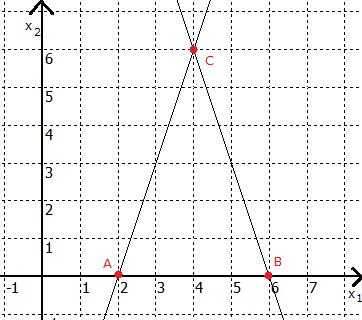
\includegraphics{images/triangle.png} \\

Sei $\alpha x + \beta$ eine komponentenweise positiv-affine Transformation von $x \in \mathbb{R}^2$, d.h.
$\alpha > 0$ und $\beta \in \mathbb{R}^2$. Wir wenden diese Transformation auf $A, B$ und $C$ an: \\

\begin{itemize}
\item{$A' = \alpha A + \beta = (\alpha_1 a_1 + \beta_1, 0 + \beta_2)$}
\item{$B' = \alpha B + \beta = (\alpha_1 \cdot (a_1 + c) + \beta_1, 0 + \beta_2$)}
\item{$C' = \alpha C + \beta = (\alpha_1 \cdot (a_1 + \frac{c}{2}) + \beta_1, \alpha_2 c_2 + \beta_2$)}
\end{itemize}

Wir stellen fest: \\

\begin{itemize}
\item{$A'$ und $B'$ haben beide den $x_2$-Wert $\beta_2 \Rightarrow A'$ und $B'$ liegen auf der Parallele
zur $x_1$-Achse durch $(0, \beta_2)$. $\overline{A'B'}$ ist die Basis des gleichschenkligen Dreiecks.}
\item{Die Distanz zwischen $A'$ und $B'$ beträgt $\alpha_1 \cdot (a_1 + c) + \beta_1 - (\alpha_1 a_1 +
\beta_1) = \alpha_1 \cdot c$. Die Differenz der $x_1$-Werte von $A$ und $C$ beträgt $\alpha_1 \cdot (a_1 +
\frac{c}{2}) + \beta_1 - (\alpha_1 a_1 + \beta_1) = \alpha_1 \cdot \frac{c}{2}$. Das ist genau
die Hälfte der Differenz der $x_1$-Werte von $A'$ und $B' \Rightarrow C'$ liegt auf der Mittelsenkrechten
zu $\overline{A'B'}$.}
\end{itemize}

Da $A'B'$ parallel zur $x_1$-Achse ist und $C'$ auf der Mittelsenkrechten zu $A'B'$ liegt, ist $A'B'C'$
ein gleichschenkliges Dreieck, dessen Basis auf einer Parallelen zur $x_1$-Achse liegt. \clearpage

\exercise{1.2}{Characterization of Nash-solutions in bargaining games}
Let $(S, d)$ with $S\subset \Real^2$ be a bargaining game. 
We want to show that $y\in S$ is 
a Nash-solution, that is\footnote{
  We introduce additional notation for rectangles (``2D-intervals''): 
  $[a, b] := \setPredicate{x \in \Real^2}{a \leq x \leq b}$, and denote the area 
  of a rectangle by $\vol[a, b]$.}
\[
  y = \mathcal{N}(S, d) 
   := \argmax_{s\in S}\vol[d, s] 
   := \argmax_{s\in S}(s_2 - d_2)(s_1 - d_1)
\] 
if and only if the following three conditions hold:
\begin{itemize}
  \item[(i)] $y\in PO(S) := \setPredicate{s\in S}{
    \forall t \in S:\quad t \geq s \Rightarrow t = s
  }$
  \item[(ii)] $y \gg d$
  \item[(iii)] $S$ is contained in one of the closed half-planes
    delimited by the line through the points $y$ and $(d_1 + 2(y_1 - d_1), d_2)$.
    \emph{
      (The original formulation of the same statement seemed
      awkward. To be precise: it was wrong, because it was not told where the
      base of the triangle is supposed to be. 
      No existence-quantor is needed here: the line is uniquely 
      determined by the ``isosceles triangle''-property, one only has to 
      check whether $S$ is completely on one side of this line or not).
    }
\end{itemize}
Without loss of generality we can assume that $d=(0,0)$.

First, we show that if $y=\mathcal{N}(S, d)$, then all three properties hold.
\begin{itemize}
  \item[(i)] Suppose $z\in S$ with $z\geq y$. Suppose for the sake of 
  contradiction that $z\neq y$. Then either $z_1 > y_1$ or $z_2 > y_2$.
  Either way:
  \[
    \vol[d, z] = (z_1 - d_1)(z_2 - d_2) > (y_1 - d_1)(y_2 - d_2) = \vol[d, y],
  \]
  which is a contradiction to the definition of $y$.
  Therefore it must hold for all $z\in S$:
  \[
    z\geq y \Rightarrow z = y,
  \]
  which means that $y\in PO(S)$.
  \item{(ii)} By the non-degeneracy assumption there must be an $s\in S$ such
  that $s \gg d$. By definition of $y$ it must hold:
  \[
    \vol[d, y] \geq \vol[d, s] = (d_1-s_1)(d_2-s_2) > 0,
  \]
  therefore both $(y_1 - d_1)$ and $(y_2-d_2)$ must be positive, that is
  $y\gg d$.
  \item{(iii)} Notice that the normal vector for the line through $y$ and
  $(2y_1, 0)$ is given by: 
  \[
    n := ((2y_1, 0) - y)^\perp = (2y_1-y_1, -y_2)^\perp = (y_2, y_1).
  \]
  Now 
  suppose for the sake of contradiction that there exists an $s\in S$ such that
  \footnote{
    We use $\bullet$ to denote the usual scalar product in $\Real^2$.
  }:
  \[ 
    (s - y)\bullet n > 0.
  \]
  Since $S$ is assumed to be convex, all points between $y$ and $s$ are also
  contained in $S$. Let's see how the area of the rectangle changes as we 
  move from $y$ to $s$:
  \begin{align*}
    &\rPar{\dd{}{t}\vol[d, (1-t)y + ts]}\vert_{t = 0} \\
      &\vspace{1em}=
      \rPar{\dd{}{t}((1-t)y_1 + t s_1)((1-t)y_2 + t s_2)}\vert_{t=0} \\
      \vspace{1em}
      &\vspace{1em}=
      \rPar{
        (-y_1 + s_1)((1-t)y_2 + t s_2)+((1-t)y_1 + t s_1)(-y_2 + s_2)
      }\vert_{t=0} \\
      &\vspace{1em}= 
      (-y_1 + s_1) y_2 + y_1 (-y_2 + s_2) \\
      &\vspace{1em}=
      (s-y)\bullet n \\
      &\vspace{1em}
      > 0.
  \end{align*}
  Therefore, there must exist some $\epsilon > 0$ such that 
  \[
    \vol[d, (1-\epsilon)y + \epsilon s] > \vol[d, y],
  \]
  which is a contradiction to the definition of $y$. Therefore, there can not
  be such an $s$, therefore:
  \[
    \forall\, s\in S: (s-y)\bullet n \leq 0,
  \]
  this is exactly what it means that the entire set $S$ is contained in one
  of the half-planes.
\end{itemize}

Now we have to prove the other direction: starting with the three properties
(i)-(iii), we have to show that $y$ is a Nash-solution. So, let the three
properties hold. First, we show that for all $s\in S$ it holds:
\[
  (s-y)\bullet n \leq 0. \quad\quad\quad (\ast)
\]
Notice that this does not directly follow from (iii), because in (iii) we could
also have a $\geq$ instead of $\leq$. To show that this must be $\leq$, we need
the property (ii):
\[
  (d - y)\bullet n = (-y_1, -y_2) \bullet (y_2, y_1) = -2y_1 y_2 < 0.
\]
Now from this we can conclude using (iii) that for all $s$ the inequality 
$(\ast)$ holds.
From (i) we can conclude that for all $s$ either both $(s_1 - y_1)$ and
$(s_2 - y_2)$ are $0$, or at least one of these expressions is negative,
let's call this property $(\dagger)$.
Either way, together with $(\ast)$ we obtain:
\begin{align*}
\vol[d,s] 
  =& s_1 s_2 \\
  =& (y_1 + (s_1 - y_1))(y_2 + (s_2 - y_2)) \\
  =& y_1 y_2 + (s_1 - y_1)y_2 + y_1(s_2 - y_2) + (s_1-y_1)(s_2 - y_2) \\
  =& y_1 y_2 + (s - y)\bullet n + (s_1 - y_1)(s_2 - y_2) \\
  \overset{\ast}\leq& y_1y_2 + (s_1 - y_1)(s_2-y_2) \\
  \overset{\dagger}\leq& y_1 y_2 = \vol[d, y].
\end{align*}
This means that $y=\mathcal{N}(S, d)$.

Both implications together imply the claimed equivalence.
\hfill \qed

\exercise{12.3}{Nash-L\"osungen}

\subexercise{a}
Wir zeigen, dass $(\frac{3}{4}, \frac{3}{4})$ die Nash-Lösung für das Spiel $(S, d)$ ist. \\

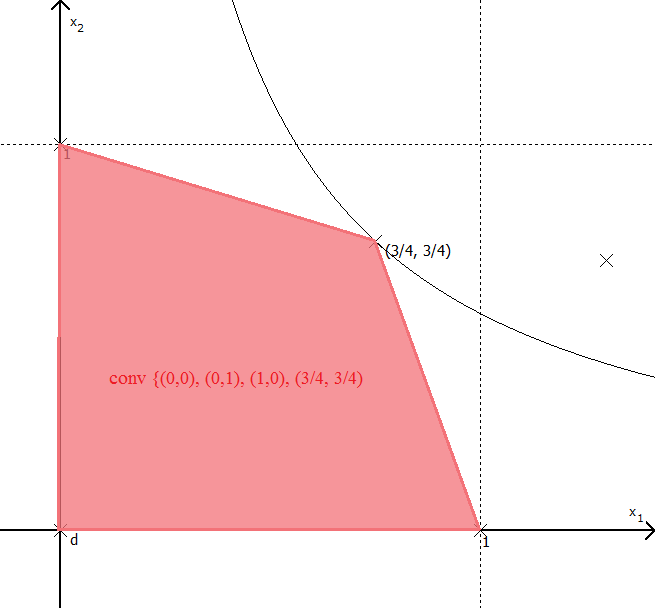
\includegraphics[width=12cm]{images/3a.png} \\

Dazu zeigen wir einfach, dass $x =(\frac{3}{4}, \frac{3}{4})$ die Alternative $x \in S$ ist, welche die Fläche
des Rechtecks mit unterer linker Ecke $d$ und oberer rechter Ecke $x$ maximiert. \\

In der Abbildung ist neben $S$ noch ein Teil der Funktion $x_2(x_1) = (\frac{3}{4})^2 \cdot \frac{1}{x_1}$
eingezeichnet, sprich dies sind genau die Punkte $(x_1, x_2)$ mit $x_1 \cdot x_2 = (\frac{3}{4})^2$. Für die
Punkte auf dieser Kurve ist der Flächeninhalt des Rechtecks mit unterer linker Ecke $d$ und oberer Rechter
Ecke $x = (x_1, x_2)$ genau $(\frac{3}{4})^2$. \\

Für $x$ oberhalb dieser Kurve ist der Flächeninhalt größer, für $x$ unterhalb kleiner. Da die Kurve genau durch
$(\frac{3}{4}, \frac{3}{4})$ verläuft und $S$ mit Ausnahme von $(\frac{3}{4}, \frac{3}{4})$ komplett unterhalb der
Kurve liegt, ist $\mathcal{N}(S, d) = (\frac{3}{4}, \frac{3}{4})$ die Nash-Lösung für dieses Spiel. \clearpage

\subexercise{b}
Die Nash-Lösung für dieses Spiel findet sich im Buch von \textsl{Maschler, Solan} und \textsl{Zamir}, wo auf
Seite 642 genau dieses Beispiel als Kritik an der Nash-Lösung aufgeführt wird. \\

\begin{figure}[h!]
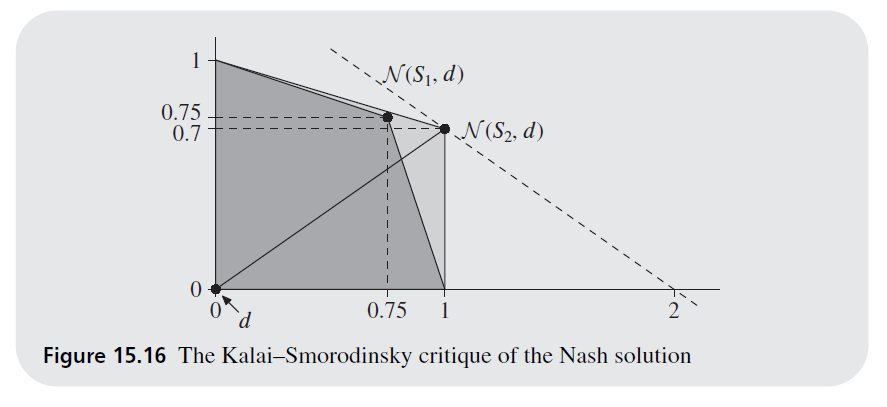
\includegraphics[width=1\textwidth]{images/3b.png}
\caption{entnommen aus \textsl{Maschler, Solan, Zamir}: Game Theory}
\end{figure}

Dort heißt es:
\begin{quotation}
[...] Since the bargaining game $(S_1,(0,0))$ is symmetric, $\mathcal{N}(S_1,(0,0)) = (0.75, 0.75)$. By
drawing an equilateral triangle whose vertices are $(0,0), (1,0.7), (2,0)$ (see Figure 15.16) and
using Theorem 15.20, we deduce that $\mathcal{N}(S_2,(0,0) = (1,0.7)$. [...]
\end{quotation}

Theorem 15.20 ist genau der Satz, welcher in Aufgabe 2 bewiesen wurde. Damit ist $\mathcal{N}(S_2,
(0,0) = (1,0.7)$ die Nash-Lösung für dieses Spiel.

\end{document}